\documentclass{math}

\usepackage{tikz}

\geometry{letterpaper, margin=0.5in}

\title{Boundary Value Problems: Homework 6}
\author{Alvin Lin}
\date{August 2018 - December 2018}

\begin{document}

\maketitle

\subsection*{Problem 1}
Write the Fourier cosine series and the Fourier sine series for
\( f(x) = \cos(x), 0<x<\pi \).
\begin{align*}
  a_0 &= \frac{2}{\pi}\int_{0}^{\pi}\cos(x)\diff{x} \\
  &= \frac{2}{\pi}\bigg[\sin(x)\bigg]_{0}^{\pi} \\
  &= \frac{2}{\pi}(\sin(\pi)-\sin(0)) \\
  &= 0 \\
  a_n &= \frac{2}{\pi}\int_{0}^{\pi}f(x)\cos(\frac{n\pi x}{\pi})\diff{x} \\
  &= \frac{2}{\pi}\int_{0}^{\pi}\cos(x)\cos(nx)\diff{x} \\
  &= \frac{2}{\pi}\int_{0}^{\pi}\frac{1}{2}\bigg[
    \cos(x-nx)+\cos(x+nx)\bigg]\diff{x} \\
  &= \frac{1}{\pi}\bigg[
    \frac{1}{1-n}\sin((1-n)x)+\frac{1}{1+n}\sin((1+n)x)\bigg]_{0}^{\pi} \\
  &= 0 \\
  b_n &= \frac{2}{\pi}\int_{0}^{\pi}f(x)\sin(\frac{n\pi x}{\pi})\diff{x} \\
  &= \frac{2}{\pi}\int_{0}^{\pi}\cos(x)\sin(nx)\diff{x} \\
  &= \frac{2}{\pi}\int_{0}^{\pi}\frac{1}{2}\bigg[
    \sin(x+nx)-\sin(x-nx)\bigg]\diff{x} \\
  &= \frac{1}{\pi}\bigg[
    \frac{-1}{1+n}\cos(x+nx)+\frac{1}{1-n}\cos(x-nx)\bigg]_{0}^{\pi} \\
  &= \frac{1}{\pi}\bigg[
    \frac{-\cos((n+1)\pi)}{1+n}+
    \frac{\cos((n-1)\pi)}{1-n}+
    \frac{\cos(0)}{1+n}-
    \frac{\cos(0)}{1-n}
  \bigg] \\
  &= \frac{1-\cos((1+n)\pi)}{(1+n)\pi}+\frac{\cos((1-n)\pi)-1}{(1-n)\pi} \\
  FCS &= 0 \\
  FSS &= \sum_{n=1}^{\infty}
    \left(
      \frac{1-\cos((1+n)\pi)}{(1+n)\pi}+\frac{\cos((1-n)\pi)-1}{(1-n)\pi}
    \right)\sin(nx)
\end{align*}

\subsection*{Problem 2}
Find the Fourier cosine series for \( f(x) = x, 0\le x\le \pi \). If the
series represents \( f(x) \) on the given interval, show graphically the
function represented by the series for all \( x \).
\begin{align*}
  a_0 &= \frac{2}{\pi}\int_{0}^{\pi}x\diff{x} \\
  &= \frac{2}{\pi}\bigg[\frac{x^2}{2}\bigg]_{0}^{\pi} \\
  &= \frac{2}{\pi}\bigg[\frac{\pi^2}{2}-0\bigg] \\
  &= \pi \\
  a_n &= \frac{2}{\pi}\int_{0}^{\pi}x\cos(\frac{n\pi x}{\pi})\diff{x} \\
  u = x \quad \diff{u} &= \diff{x} \quad \diff{v} = \cos(nx) \quad
    v = \frac{-\sin(nx)}{n} \\
  &= \frac{2}{n}\left[\left[\frac{x\sin(nx)}{n}\right]_{0}^{\pi}-
    \int_{0}^{\pi}\frac{1}{n}\sin(nx)\diff{x}\right] \\
  &= \frac{2}{n}\left[\frac{\pi\sin(n\pi)}{n}-
    \left[\frac{-\cos(nx)}{n^2}\right]_{0}^{\pi}\right] \\
  &= \frac{2}{n}\left[\frac{\pi\sin(n\pi)}{n}-
    \left[\frac{-\cos(n\pi)}{n^2}+\frac{\cos(0)}{n^2}\right]\right] \\
  &= \frac{2\pi\sin(n\pi)}{n^2}-\frac{1-\cos(n\pi)}{n^3} \\
  f(x) &\sim \frac{\pi}{2}+\sum_{n=1}^{\infty}\left(
    \frac{2\pi\sin(n\pi)}{n^2}-\frac{1-\cos(n\pi)}{n^3}\right)\cos(nx)
\end{align*}
\begin{center}
  \begin{tikzpicture}
    \draw[thick,<->] (-3,0) -- (3,0) node[below] {\( x \)};
    \draw[thick,<->] (0,-3) -- (0,3) node[left] {\( y \)};
    \draw[very thick,red] (-2,0) -- (-1,1) -- (0,0) -- (1,1) -- (2,0);
  \end{tikzpicture}
\end{center}

\subsection*{Problem 3}
If \( f(x) = x^2, 0<x<\pi \), find the Fourier sine series and draw a graph
of the function with its periodic extension.
\begin{align*}
  b_n &= \frac{2}{\pi}\int_{0}^{\pi}x^2\sin(\frac{n\pi x}{\pi})\diff{x} \\
  & \text{by integral table} \\
  &= \frac{2}{\pi}\bigg[
    \frac{(2-n^2x^2)\cos(nx)-2nx\sin(nx)}{n^3}\bigg]_{0}^{\pi} \\
  &= \frac{2}{\pi}\bigg[
    \frac{(2-n^2\pi^2)\cos(n\pi)-2n\pi\sin(n\pi)}{n^3}-
    \frac{(2-0)\cos(0)-0}{n^3}
  \bigg] \\
  &= \frac{2}{\pi}\bigg[\frac{(2-n^2\pi^2)\cos(n\pi)-2}{n^3}\bigg] \\
  f(x) &\sim \sum_{n=1}^{\infty}
    \frac{2}{\pi}\bigg[\frac{(2-n^2\pi^2)\cos(n\pi)-2}{n^3}\bigg]\sin(nx) \\
\end{align*}
\begin{center}
  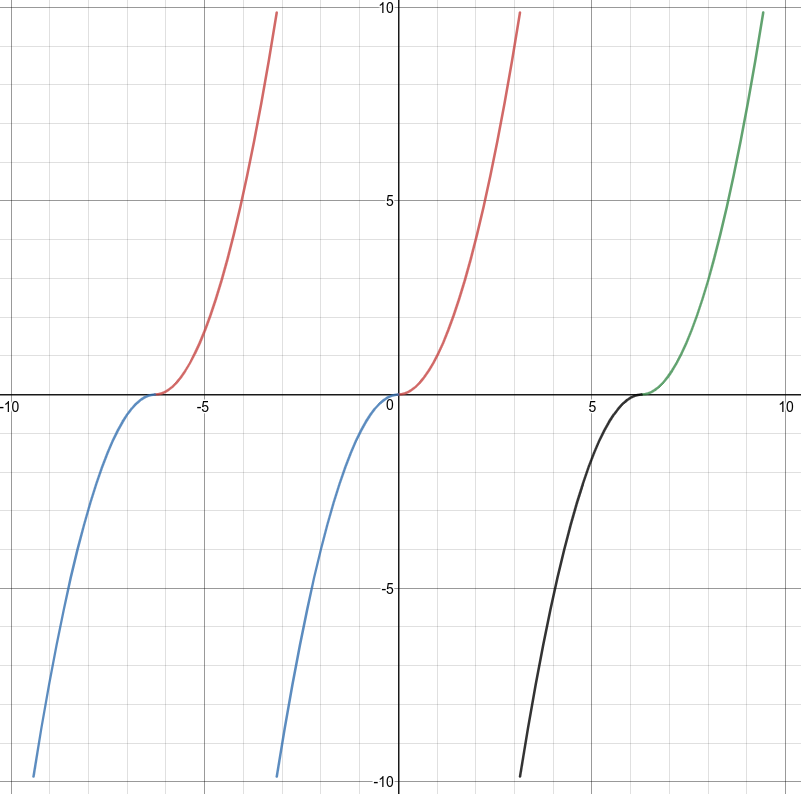
\includegraphics[width=12cm]{assets/hw_06_graph.png}
\end{center}

\subsection*{Problem 4}
Exercise 12: Find the double Fourier series if
\[ f(x,y) = xy^2, -\pi<x<\pi, \pi<y<\pi \]
Since the function is odd in \( x \) and even in \( y \), the coefficients
\( a_{mn}, b_{mn}, d_{mn} \) are zero.
\begin{align*}
  c_{mn} &= \frac{1}{\pi^2}\int_{-\pi}^{\pi}\int_{-\pi}^{\pi}xy^2
    \sin(\frac{m\pi x}{\pi})\cos(\frac{n\pi y}{\pi})\diff{x}\diff{y} \\
  &= \frac{1}{\pi^2}\int_{-\pi}^{\pi}x\sin(mx)\diff{x}
    \int_{-\pi}^{\pi}y^2\cos(ny)\diff{y} \\
  &= \frac{1}{\pi^2}
    \bigg[\frac{\sin(mx)-mx\cos(mx)}{m^2}\bigg]_{-\pi}^{\pi}
    \bigg[\frac{(n^2y^2-2)\sin(ny)+2ny\cos(ny)}{n^3}\bigg]_{-\pi}^{\pi} \\
  &= \frac{1}{\pi^2}
    \bigg[
      \frac{\sin(m\pi)-m\pi\cos(m\pi)}{m^2}-
      \frac{\sin(-m\pi)+m\pi\cos(-m\pi)}{m^2}
    \bigg] \\
  &\quad \bigg[
    \frac{(n^2\pi^2-2)\sin(n\pi)+2n\pi\cos(n\pi)}{n^3}-
    \frac{(n^2\pi^2-2)\sin(-n\pi)-2n\pi\cos(-n\pi)}{n^3}
  \bigg] \\
  &= \frac{1}{\pi^2}\bigg[\frac{-2m\pi\cos(m\pi)}{m^2}\bigg]
    \bigg[\frac{4n\pi\cos(n\pi)}{n^3}\bigg] \\
  &= \frac{-8\cos(m\pi)\cos(n\pi)}{mn^2} \\
  f(x,y) &\sim \frac{1}{2}\sum_{m=1}^{\infty}
    \bigg[c_{m0}\sin(\frac{m\pi x}{K})\bigg]+
    \sum_{m=1}^{\infty}\sum_{n=1}^{\infty}
    \bigg[c_{mn}\cos(\frac{n\pi y}{L})\bigg]\sin(\frac{m\pi x}{K}) \\
  &= 0+\sum_{m=1}^{\infty}\sum_{n=1}^{\infty}
    \bigg[\frac{-8\cos(m\pi)\cos(n\pi)\cos(ny)}{mn^2}
    \bigg]\sin(mx)
\end{align*}
Exercise 13: Find the double Fourier series if
\[ f(x,y) = x^2y^2, -\pi<x<\pi, -\pi<y<\pi \]
Since the function is even in \( x \) and \( y \), the coefficients
\( b_{mn}, c_{mn}, d_{mn} \) are zero.
\begin{align*}
  a_{mn} &= \frac{1}{\pi^2}\int_{-\pi}^{\pi}\int_{-\pi}^{\pi}x^2y^2
    \cos(mx)\cos(ny)\diff{x}\diff{y} \\
  &= \frac{1}{\pi^2}\int_{-\pi}^{\pi}x^2\cos(mx)\diff{x}
    \int_{-\pi}^{\pi}y^2\cos(ny)\diff{y} \\
  &= \frac{1}{\pi^2}
    \bigg[\frac{(m^2x^2-2)\sin(mx)+2mx\cos(mx)}{m^3}\bigg]_{-\pi}^{\pi}
    \bigg[\frac{(n^2y^2-2)\sin(ny)+2ny\cos(ny)}{n^3}\bigg]_{-\pi}^{\pi} \\
  &= \frac{1}{\pi^2}
    \bigg[
      \frac{(m^2\pi^2-2)\sin(m\pi)+2m\pi\cos(m\pi)}{m^3}-
      \frac{(m^2\pi^2-2)\sin(-m\pi)-2m\pi\cos(m\pi)}{m^3}
    \bigg]\dots \\
  &= \frac{1}{\pi^2}
    \bigg[\frac{4m\pi\cos(m\pi)}{m^3}\bigg]
    \bigg[\frac{4n\pi\cos(n\pi)}{n^3}\bigg] \\
  &= \frac{16\cos(m\pi)\cos(n\pi)}{(mn)^2} \\
  f(x,y) &\sim \frac{a_{00}}{4}+\frac{1}{2}\sum_{n=1}^{\infty}a_{0n}\cos(ny)+
    \frac{1}{2}\sum_{m=1}^{\infty}a_{m0}\cos(mx)+
    \sum_{m=1}^{\infty}\sum_{n=1}^{\infty}\bigg[a_{mn}\cos(ny)\bigg]\cos(mx) \\
  &?= \sum_{m=1}^{\infty}\sum_{n=1}^{\infty}\bigg[
    \frac{16\cos(m\pi)\cos(n\pi)\cos(ny)}{(mn)^2}\bigg]\cos(mx)
\end{align*}

\begin{center}
  If you have any questions, comments, or concerns, please contact me at
  alvin@omgimanerd.tech
\end{center}

\end{document}
